\documentclass[11pt]{amsart}
\usepackage{geometry}                % See geometry.pdf to learn the layout options. There are lots.
\geometry{letterpaper}                   % ... or a4paper or a5paper or ... 
\usepackage[parfill]{parskip}    % Activate to begin paragraphs with an empty line rather than an indent
\usepackage{graphicx}
\usepackage{hyperref}
\usepackage{amssymb}
\usepackage{multirow}
\usepackage{fancyvrb}
\usepackage{color}
\definecolor{comment_color}{rgb}{0.6, 0.6, 0.6}
\newcommand{\pyc}[1]{\textcolor{comment_color}{#1}}


\title{Making and Working with Movies}
\author{Gruppo D'Irvino}
%\date{}                                           % Activate to display a given date or no date

\begin{document}
\maketitle
\section{Introduction}
This is a short guide on taking video in the lab.
It is primarily focussed on working with the \emph{Vision Research} High-Speed Cameras, but the reference information should be useful to anyone interested in taking videos for data analysis.
The source of this document should be available in the \texttt{guide} directory of the \emph{cine} repository.

The sections on handling data require a reasonably complete scientific \emph{Python} distribution, or at least one which includes the \emph{Scipy} and \emph{Python Imaging Library} (PIL) modules.
For an academic environment, the most convenient choice is the \href{http://www.enthought.com/}{\emph{Enthought Python Distribution}}, which is free to academic users (recent versions can usually be found on {\bf immenseirvine}).

This guide will make use of Mac \emph{OS X}, but the \emph{cine} module and command line tools should work in \emph{Windows} or \emph{Linux} without modification. 

\section{Imaging Basics}
\begin{figure}
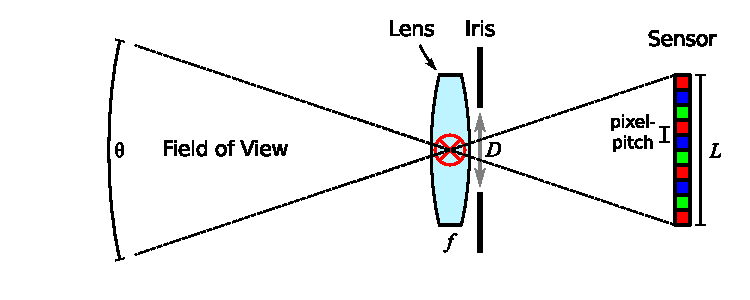
\includegraphics{figures/camera.pdf}
\caption{A schematic of a camera, with the sensor size, $L$, iris diameter, $D$ and focal length, $f$ labeled.}
\label{fig:camera}
\end{figure}

At its most basic level, a camera consists of an image sensor and a lens (Fig. \ref{fig:camera}).
All other things being equal, a larger sensor usually provides better image quality, especially in low light situations.
For this reason, the \emph{Phantom} cameras have very large sensors, especially for their resolution, to maximize light sensitivity and minimize exposure times.
%Many other things affect the final image, including the choice of lens focal length/aperture and frame exposure time.
A practical discussion of the most important imaging concepts follows, in terms of both camera hardware and the resulting digital data.



\subsection{Lens Choice and Focal Length}
In the lab, you will primarily find two types of lenses: F-mount (for large lenses on the SLRs or Phantoms) and C-mount (on small USB or Ethernet cameras). 
Adapters exist for putting F-mount lenses to C-mount, although you will likely not get great image quality if the pixel pitch is less than 5 $\mu$m, as is commonly the case for small, high-resolution cameras ($\gtrsim$ 1 megapixel).
Mounting C-mount lenses of F-mount cameras is not possible because F-mount is designed for larger sensors.

The focal length of the lens changes the field of view of the camera in the following way:
$$
\theta = 2\ \sin^{-1}\frac{d_i}{2L} \sim \frac{f}{L},
$$
where $\theta$ is the angular field of field, $f$ is the lens focal length, $d_i$ is the image distance (distance from lens center to image plane, and $L$ is the sensor size (width or height).
Typically $d_i \sim f$, unless the object is very close to the camera.
A `longer' lens, with larger focal length, will have a smaller field of view.
{\bf A smaller field of view is preferable for data analysis, since the resulting image will have less distortion.}

\subsection{Aperture}
\begin{figure}
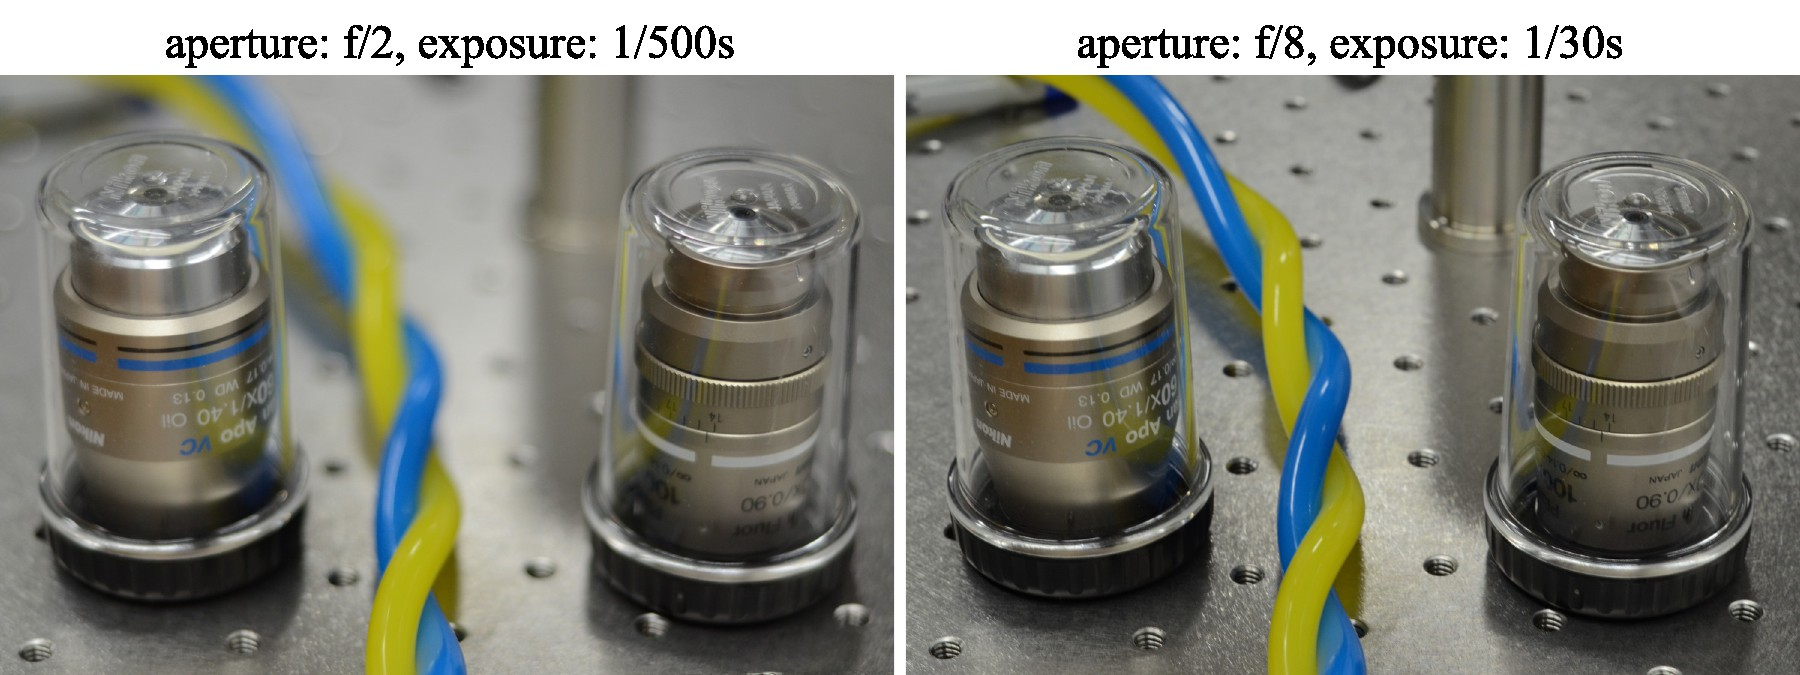
\includegraphics{figures/aperture-300dpi.jpg}
\caption{
An picture of two microscope objectives on an optical table, showing the effect of aperture on an image.  
The large aperture image (left) has less depth of field, meaning the out of focus areas are more blurred.
To keep the brightness the same, the exposure time needed to be adjusted by a factor of $\sim$16 to compensate for the aperture.
}
\label{fig:blur}
\end{figure}

Lenses fall into two categories: `zoom' lenses, with adjustable focal lengths, and `prime' lenses, with a single focal length.
Prime lenses usually have slightly better image quality (sharpness and contrast) and larger apertures, at the expense of convenience.
Prime lenses are also usually easier to manually focus, due both to the larger aperture as well as a (typically) better focussing mechanism.

The lens aperture if the effective opening size at the optical center of the lens, which can be adjusted with an iris.
{\bf A larger aperture will let in more light, allowing for shorter exposure times, at the expense of `depth-of-field,' which is a measure of the range of distances that are in focus (Fig. \ref{fig:blur}).}
The size of the aperture is usually listed as a fraction of the lens focal length: for example, for a lens with a focal length of $f=100$ mm, $f/2$ corresponds to a 50mm diameter aperture, and $f/8$ corresponds to a 12.5mm aperture.
Larger aperture lenses (smaller f-number) are often referred to as `fast,' because they allow for shorter exposures.

Note that the amount of light transmitted by the lens goes like the \emph{square} of the aperture radius; thus $f/2$ is twice as bright as $f/2.8$, which is twice again as bright as $f/4$.
In photography each factor of two increase in exposure is referred to as a `stop,' for this reason the aperture values labeled on a lens are spaced by $\sqrt{2}$.

For an F-mount prime lenses, $f/1.4$--$f/2.8$ are commonly available, with $f/2.8$ being most common. %\footnote{Excepting $f=50$mm, for which $f/1.8$ and $f/1.4$ lenses are cheap and common.}.

\subsubsection{Depth of field.}


The depth-of-field can be determined from the lens equation, but in the limit that the object is relatively close to the camera (Fig. \ref{fig:dof}):
$$
\Delta \approx \frac{2 \left(1 + m\right) N \delta}{m^2},
$$
where $\Delta$ is the total range of depths that are ``in focus'', $\delta$ is the acceptable blurring, $m$ is the magnification and  $N$ is the F-number of the lens.
(This approximation should be fine for pretty much any lab experiment.)
Commonly, the acceptable blur, $\delta$, will be set to the pixel-pitch, since the camera can not resolve finer details.
A brief depth of field table for $\delta=20\mu$m is shown below; note that the pixel pitch is 22$\mu$m on the \emph{Phantom V12} and 28$\mu$m of the \emph{V1610}.

\begin{figure}
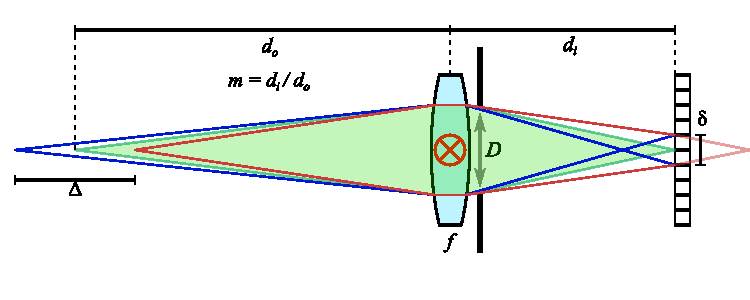
\includegraphics{figures/dof.pdf}
\caption{Determining the depth of field, $\Delta$.  The image magnification, $m$, is given by the ratio between the image distance, $d_i$ and object distance, $d_o$.  The maximum amount of in-focus range in the object plane, $\Delta$ is dependent on the aperture size, $D$, and the allowable amount of defocussing, $\delta$.  By using the lens equation, $f^{-1} = d_i^{-1} + d_o^{-1}$, one can determine the amount of blur in the image plane for a defocussed object; the small defocus expansion gives: $\Delta \approx \frac{2 \left(1 + m\right) N \delta}{m^2}$.}
\label{fig:dof}
\end{figure}

\begin{centering}
\begin{tabular}{c|c|c|c|c|c|c|c}
{\bf $\boldsymbol{\delta=20\mu}$m}&\multicolumn{2}{|c|}{mm/pixel}&\multicolumn{3}{|c|}{Depth-of-Field (mm)}&\multicolumn{2}{|c}{Subject-sensor distance (mm)}\\
\hline
Magnification ($m$)&V12&1610&$f/2$&$f/4$&$f/8$&$f=50$mm&$f=100$mm\\
\hline
1:100&2.2&2.8&800&1600&3200&5100&10200\\
1:30&0.66&0.84&75&150&300&1600&3200\\
1:10&0.20&0.28&9&18&35&605&1210\\
1:3&0.066&0.084&1&2&4&267&533\\
1:1&0.022&0.0028&0.15&0.3&0.6&200&400\\
\end{tabular}
\end{centering}

\subsubsection{Diffraction}
If the aperture is too small, optical diffraction can limit the resolution.
For a given f-number, $N$, the smallest focussed spot a lens can produce is:
$$
A \sim 1.22 \lambda N,
$$
where $A$ is the approximate spot diameter, $\lambda$ is the wavelength of light ($\lambda \sim0.5\mu$m for visible light).
When this spot size becomes comparable to the pixel pitch, blurring will be visible even for optimally focussed objects.
{\bf For the \emph{Phantom} cameras, diffraction is generally not a problem}: most lenses have a minimum aperture of $f/22$ or $f/32$, and the diffraction limited spot size just barely approaches the pixel size at these apertures.
For the \emph{Nikon D7000}, the pixel pitch is $\sim 5\mu$m, and for small USB or Ethernet cameras it is in the range 2--5$\mu$m; in this case diffraction becomes relevant at $\sim f/4$--$f/11$. 

Note that lenses are not guaranteed to be diffraction limited at all apertures: F-mount lenses usually perform best at $f/5.6$--$f/8$ and have \emph{worse} resolution at larger apertures (smaller f-numbers) due to optical aberrations.
For this reason, a properly designed C-mount lens is preferable for miniature, high resolution cameras\footnote{Because the C-mount is designed to cover a smaller sensor, it is easier to design large aperture lenses that are diffraction limited.}.
Because of the large pixels, optical aberrations should not limit resolution on the \emph{Phantoms}.

\subsection{Exposure Time}
Shorter exposures result in less blurred images for moving objects.  
Shorter exposures are possible with larger aperture lenses, or by using a camera with a larger/more sensitive sensor.

Some small cameras have what is known as a `rolling-shutter,' which means that not all of the image is exposed at the same time.
This can result in moving objects appearing slanted or wobbly\footnote{For a good example of this, take a video with a camera phone out the window of a moving car.}; for fast moving objects `global-shutter' cameras, like the \emph{Phantoms}, should be used instead.

\subsection{Digital Video}
What does the raw data from a video file look like?
Generally you'll have a `stack' of frames in some video file format, or perhaps a bunch of image files in a directory.
These frames may be either raw or compressed -- usually compressed video is `lossy,' meaning the original data can not be exactly recovered, although `lossless' compression does exist.
{\bf Compressed formats are useful for displaying and previewing data, but should be avoided for numerical data analysis}.
Algorithms which are sensitive to high frequency information, like PIV, will give bad results when compressed data is used.

After it is extracted from the video file, each frame consists of an array of numbers, usually with a `bit-depth' of 8--16 bits (e.g. the actual range is $[0, 2^b-1] \rightarrow[0, 255]$--$[0, 65535]$).
Commonly video with 10 or 12-bit data is encountered, and almost always this is stored as 16 bits in memory: this means the actual data has a range of $[0,1023]$ or $[0,4095]$, and the extra 4--6 bits are empty.
Color images have three independent `channels,' corresponding to red, green and blue\footnote{Occasionally, color images will have 4 channels.  The fourth channel is `alpha,' which is used to make partially transparent images.  This is most commonly encountered in PNG files, although TIFF and TGA files support it as well.}.
The actual number stored in the image array \emph{may or may not} be proportional to the original intensity recorded by the camera; see the section on gamma below.

Still images and video can be stored in many formats; a brief description of some common digital formats and their {\bf typical} is below.
%Some of these formats are capable doing more than I describe below, but I will only mention the most common usage.
\begin{itemize}
\item {\bf TIFF.} ``Tagged Image File Format.''  A rather antiquated image file format which is widely used in scientific imaging, because it has good support for high bit-depth images.  Commonly used to store image stacks, i.e. videos.  Useful for moving data to \emph{ImageJ}, or other 3rd party software, because it is almost universally supported.  Limited to 4GB maximum file size, which can be a problem for large videos\footnote{This is due to the unfortunate choice of 32 bit data pointers in the original format design.  There are alternative related formats that work around this, but none have gained universal acceptance.}.  
%TIFF has limited support for adding meta-data, but only in predefined fields (typically this is useless in practice).
TIFF was originally designed to be used to store single images, not stacks, so if you open it in software intended for working with still images (e.g.~\emph{Photoshop} or the \emph{Python Imaging Library}) you will only get the first frame.
\item {\bf CINE.} The proprietary file format used by the Phantom Cameras.  Stores the raw video data as well as all the meta-info about the video, such as camera model, frame rate, exposure settings, etc.
\item {\bf AVI.} A video `container' format.  Used to store compressed video and/or audio, but the actual format used to store the data can be one of many options.  When used for scientific video, usually an AVI is in the \emph{MJPEG} format, which is just a bunch of JPEGs mashed together with a header (as produced by the \emph{cine} library or \emph{ImageJ}).  They are very useful for previewing data, but use of an uncompressed format is recommended for data analysis. % unless you are only interested in qualitative analysis.
\item {\bf MOV, MP4, MKV, ``Quicktime,'' etc.}  Other examples of video containers.  Usually you will find that the video in these formats is in a more compressed format, e.g. \emph{h264}, which can be many times smaller than an MJPEG video or orders of magnitude smaller than raw video.  This makes them useful for distributing video on the web or sending to a journal, but not for inter-lab scientific use.
\item {\bf PNG.}  Used for storing single images in a \emph{lossless} compressed format.  More compact than an uncompressed raw format without mangling data, but it is slower to open or save, which can be an issue when working with 100's or 1000's of images. 
\item {\bf JPEG.} (AKA JPG)  A format for storing single, compressed frames.  At high quality settings, a JPEG will be nearly indistinguishable from an uncompressed image \emph{by eye}, while being only a fraction of the original size.  Despite this, it should be avoided when possible for data analysis: just because your vision system doesn't notice the compression effects, it doesn't mean your data analysis won't.%  Usually pretty fast to save/load, because it is the most commonly used image format.
%\item {\bf TGA.} Another antiquated format, used to store single uncompressed frames.  Used internally by some of the \emph{cine} tools because it is very quick to load/save.
\end{itemize}

\subsection{Gamma Correction}
\label{sec:gamma}



The response of the human retina is more-or-less logarithmic to applied light.
Thus, when a digital image is intended to viewed by people, it is not optimal to store the image data as values which are linearly proportional to brightness.
On the other hand, digital image sensors are extremely linear, and usually the raw data captured by the camera will be proportional to the light incident on the camera.
This leads to some conflict between image data used for scientific and non-scientific purposes.

The non-linearity of image data is expressed as a `gamma' value:
$$
\frac{I}{I_{\rm max}} \propto \left(\frac{n}{n_{\rm max}}\right)^\gamma,
$$
where $I$ is captured or displayed light intensity, $n$ is the integer value stored in the image file, and $\gamma$ is the gamma value.
$I_{\rm max}$ and $n_{\rm max} = 2^b - 1$ are the maximum recorded intensity and its corresponding numeric value.
{\bf Generally, scientifically oriented cameras do not apply gamma correction (or $\boldsymbol{\gamma=1}$), while cameras intended for non-scientific imaging do ($\boldsymbol{\gamma=2.2}$).}

A computer monitor will behave as if the displayed data is nonlinear and image files from non-scientific cameras (like DLSRs) will have their data corrected accordingly, i.e. $n \propto I^{1/2.2}$.
Thus a pixel is twice as bright in reality will only have a numerical value that is $2^{1/2.2} \sim 1.37$ times as large in the image data.  
Alternatively, if you double the numerical value of a pixel on a display, it will actually emit $2^{2.2} \sim 4.6$ times as much light.

Scientific cameras, including the \emph{Phantom} cameras, will not correct the image data: implicitly $\gamma = 1$.
A pixel which is twice as bright has twice the numerical value.
Unfortunately, this means that uncorrected images from these cameras will appear overly dark and contrasty when displayed normally (Fig. \ref{fig:gamma}).
Sometimes this is useful for displaying data, but you should be aware that it is not "perceptually correct," i.e. it is related to the real image in a non-linear way.
If desired, this is relatively easy to correct with \emph{ImageJ} or the \emph{cine} library.



\begin{figure}
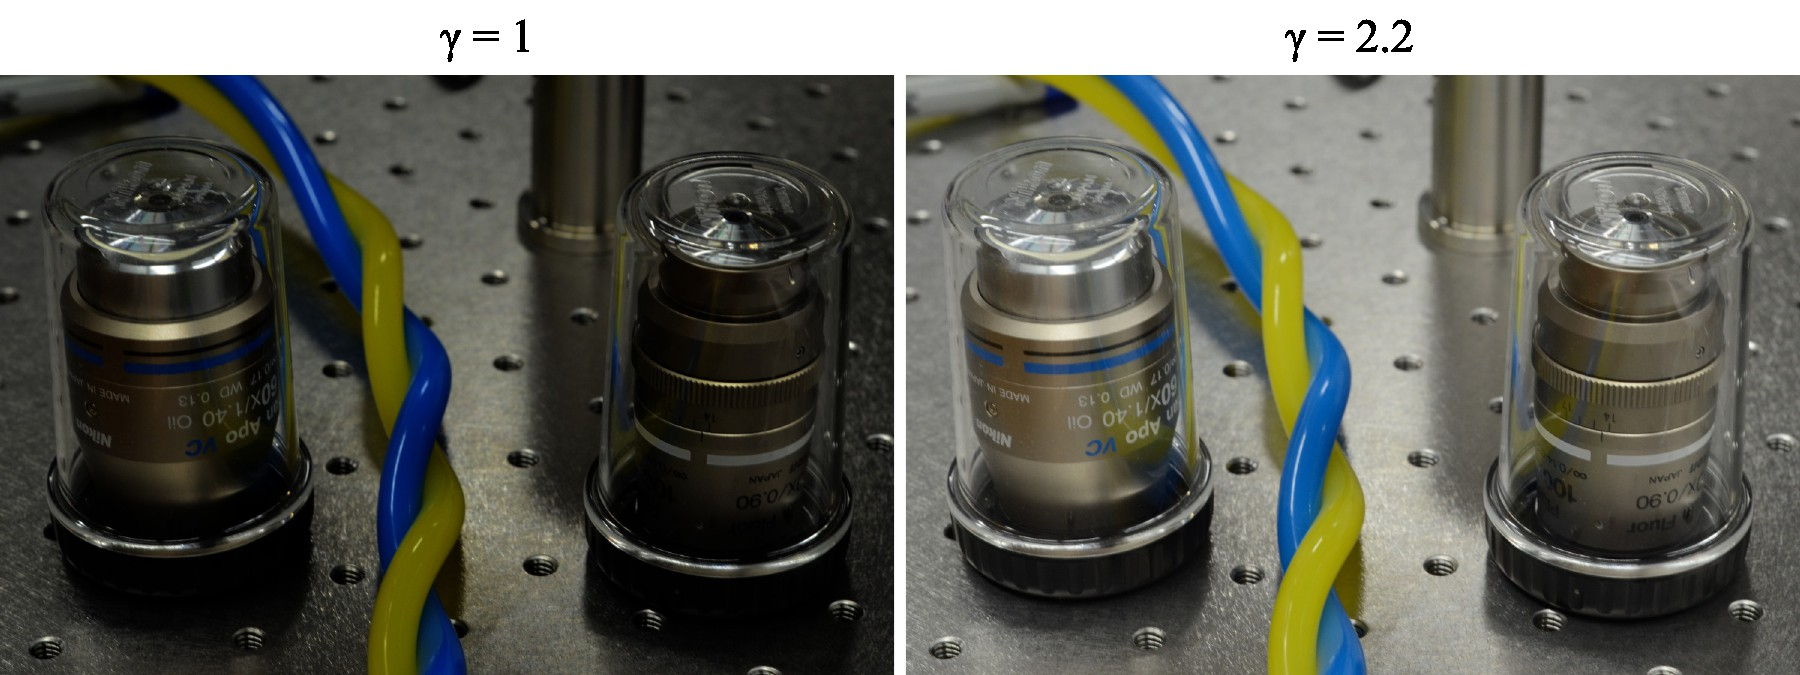
\includegraphics{figures/gamma-300dpi.jpg}
\caption{A non-gamma corrected (left) and gamma-corrected image (right).  The right image is perceptually correct, and is what you would obtain from a normal digital camera.  The image at left is what you would get from a scientific camera like the \emph{Phantom}.  Note that although the non-gamma corrected image is darker on average, the brightest spots appear the same -- the gamma effects the linearity of the brightness, not the overall scale.}
\label{fig:gamma}
\end{figure}

Note that the \emph{Phantom} cameras tend to have a slight offset in the recorded brightness: for example, on the \emph{V1610} a pure `black' frame will have a numerical value of $\sim$60 (\emph{after} a reference frame is taken)\footnote{This offset is presumably intentional, as it prevents a randomly fluctuating background from clipping to 0.  This would prevent bias when binning or doing other data processing tasks.}.
This offset should be subtracted before the gamma is applied, or else a dark grey background will be visible.

\vfill \pagebreak
\section{The CINE Package}
The \emph{cine} package is a \emph{Python} module and a set of command line tools for working with movies produced by the \emph{Phantom} software, which also includes basic classes for creating AVI and TIFF files.
The \emph{cine} library is a work in progress, but the basic usage described below should continue to work in future versions.

\subsection{Installation}
\subsubsection{OS X}
To install the package, you first need to get a copy of it.
If you are on the university network, it can be downloaded from the Irvine Group \emph{Subversion} (SVN) repository.
First open a \emph{Termnal} window, and then enter:
\begin{verbatim}
    svn co svn://immenseirvine.uchicago.edu/cine
\end{verbatim}
It should ask for a username/password, which you can get from someone in the group.
This should download the most recent version of the \emph{cine} repository.

To install it, enter the following commands in the terminal:
\begin{verbatim}
    cd cine
    ./install_osx.sh
\end{verbatim}
After a bit, the second command should ask you for your administrator password, which is required to install the package.

If a newer version is released, it can be updated with the following commands: (run from the \texttt{cine} directory)
\begin{verbatim}
    svn update
    ./install_osx.sh  
\end{verbatim}

\subsubsection{Windows}
Installation on \emph{Windows} is also simple, but you will need to get an \emph{Subversion} client first.
A good option is \href{http://tortoisesvn.net/}{\emph{Tortoise SVN}}, which integrates with file browser windows nicely.

Once you have a client, you can download the repository from:\\ \texttt{svn://immenseirvine.uchicago.edu/cine}, and then run the \texttt{install\_windows.bat} batch file in the \texttt{cine} directory to install the tools.

Depending on your \emph{Windows} settings, you may need to run this script as Administrator.
This can be done by opening a terminal by right clicking on the \emph{Command Prompt} program (in the Start menu) and selecting ``Run as Administrator''.
In the command prompt, navigate \texttt{cine} folder and run \texttt{install\_windows.bat}.

\subsection{Command Line Tools}
For simple conversion tasks, a number of simple utilities already exist for converting file types:
\begin{itemize}
\item \texttt{cine2tiff}. Convert a CINE file(s) to a TIFF file(s), and also makes a TXT file that lists some useful properties (frame rate, exposure, etc.) from the CINE.  Has no options at all -- it just does a straight conversion.
\item \texttt{cine2avi}. Covert a CINE to an AVI file.  Common options for adjusting image properties are discussed below.
\item \texttt{img2avi}. Creates an AVI from a stack of images.
\item \texttt{multicine2avi}. Creates an AVI from multiple CINEs, which are stacked side by side.
\item \texttt{cine2mp4}. Convert a CINE to an \emph{h264}-encoded MP4 file.  Requires \texttt{ffmpeg} to be available at the command line (this is most easily obtained from \href{http://www.macports.org/}{Macports}).
%\item \texttt{cine2sparse}.  Makes a SPARSE video file.  This is used as an intermediary format for the 4D viewing software, but could be useful for other projects.  The SPARSE format efficiently encodes frames that are mostly empty (black) by subtracting a background value and clipping.  Can be opened easily with the CINE library.
%\item \texttt{make\_s4d}.  Makes an S4D (sparse 3D + time) file from a CINE or SPARSE file and a 3DSETUP file.  Used for the 4D viewer.
\end{itemize}
There are also two commands (\texttt{cine2sparse} and \texttt{make\_s4d}) designed for use with the 4D viewer software, which won't be described here.

{\bf All of the commands (except for \texttt{cine2tiff}) have command line options, a list of them can be obtained by typing: \texttt{[command] --help}}.
For example:
\begin{Verbatim}[commandchars=\\\{\}, formatcom=\color{red}]
\textcolor{black}{cine2avi --help}

usage: cine2avi [-h] [-o OUTPUT] [-g GAMMA] [-f FRAMERATE] [-q QUALITY]
                [-c CLIP] [-s HIST_SKIP] [-r ROTATE]
                cines [cines ...]

Convert CINE file(s) to an AVI. Also works on TIFFs.

positional arguments:
  cines         input cine file(s), append [start:end:skip] (python slice
                notation) to filename to convert only a section

optional arguments:
  -h, --help    show this help message and exit
  -o OUTPUT     output filename, may use %s for input filename w/o extension
                or %d for input file number
  -g GAMMA      gamma of output, assumes input is gamma 1, or: I ->
                I**(1/gamma); use 2.2 to turn linear image to "natural" for
                display [default: 1]
  -f FRAMERATE  frames per second [default: 30]
  -q QUALITY    JPEG quality (0-100) [default: 75]
  -c CLIP       histogram clip, clip the specified fraction to pure black and
                pure white, and interpolate the rest; applied before gamma;
                recommended is 1E-4 - 1E-3 [default: 0]
  -s HIST_SKIP  only check every Nth frame when computing histogram clip
                [default: 5]
  -r ROTATE     amount to rotate in counterclockwise direction, must be
                multiple on 90 [default: 0]
\end{Verbatim}

\vfill \pagebreak

\subsubsection{Adjusting Images with cine2avi}
Often a video straight from the \emph{Phantom} cameras will come out dark.

\vspace{0.5cm}
\begin{tabular}{p{4in}p{2in}}
Consider the frame from the video at right, converted with:
\vspace{0.5cm}
\begin{verbatim}
cine2avi v1610_balloon.cine
\end{verbatim}
\vspace{0.5cm}
This darkness is caused by two factors: 1) the original image was slightly underexposed and 2) the gamma isn't properly adjusted (see  section \ref{sec:gamma}).
The underexposure can be corrected by rescaling the original image so that the full range of brightness values is used; the \texttt{cine2avi} command has a ``histogram clip'' option for doing this automatically!
&
\vspace{-10pt}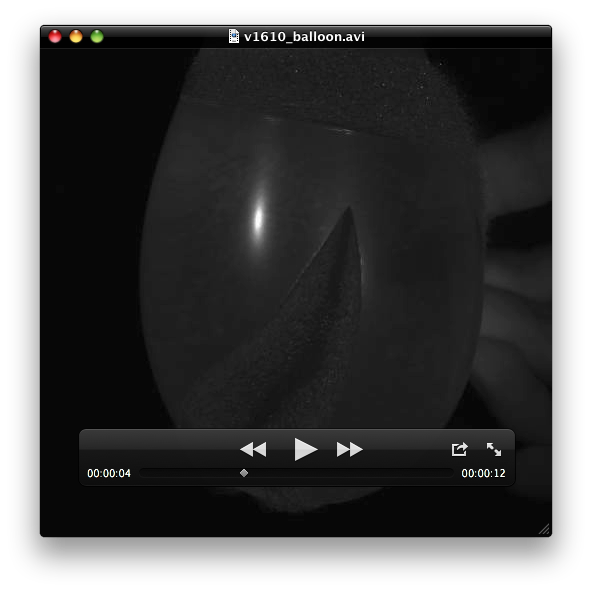
\includegraphics[width=2in]{figures/cine2avi.png}
\\
As an example, we add the histogram clip with \texttt{-c 1E-3}:
\vspace{0.5cm}
\begin{verbatim}
cine2avi v1610_balloon.cine -c 1E-3 -o %s-b.avi
\end{verbatim}
\vspace{0.5cm}
The \texttt{-c 1E-3} option specified that 0.1\% of the darkest and brightest values get clipped to pure black or white, and the rest get interpolated in between.  Specifying a larger clip, like \texttt{-c 1E-2} will make the image more contrasty, at the expense of more clipping.
We have also specified a different output name with \texttt{\%s-b.avi}, to avoid overwriting the original AVI.
&
\vspace{-10pt}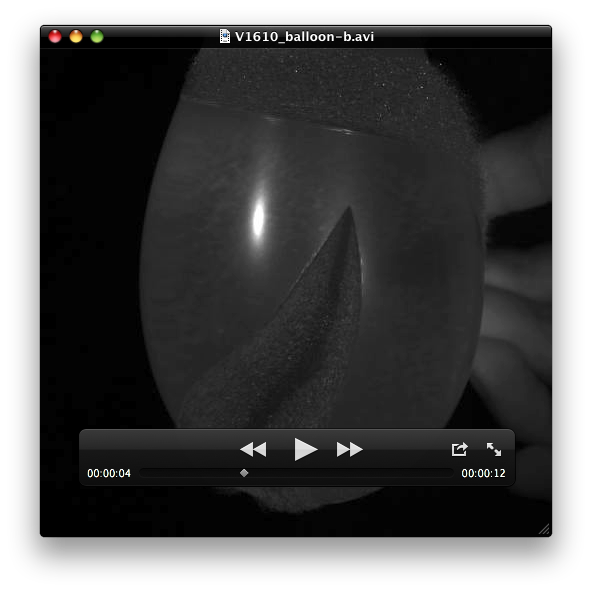
\includegraphics[width=2in]{figures/cine2avi_b.png}
\\
%We have also specified a different output name with \texttt{\%s-b.avi}, to avoid overwriting the original AVI.
%Here the \texttt{\%s} gets replaced by the original file name, so \texttt{v1610\_balloon.cine} becomes \texttt{v1610\_balloon-b.avi}.
%Specifying output filenames this way is especially useful when you have multiple inputs.
Finally, we apply some gamma correction with the \texttt{-g 2.2} option:
\vspace{0.5cm}
\begin{verbatim}
cine2avi v1610_balloon.cine -c 1E-3 -g 2.2 \
 -o %s-bg.avi
\end{verbatim}
\vspace{0.5cm}
As mentioned in the gamma correction section, videos produced by the \emph{Phantoms} usually have a slight zero-offset in the image data, so it is recommended to always use a histogram clip when applying gamma (or you will get a dark gray background).
&
\vspace{-10pt}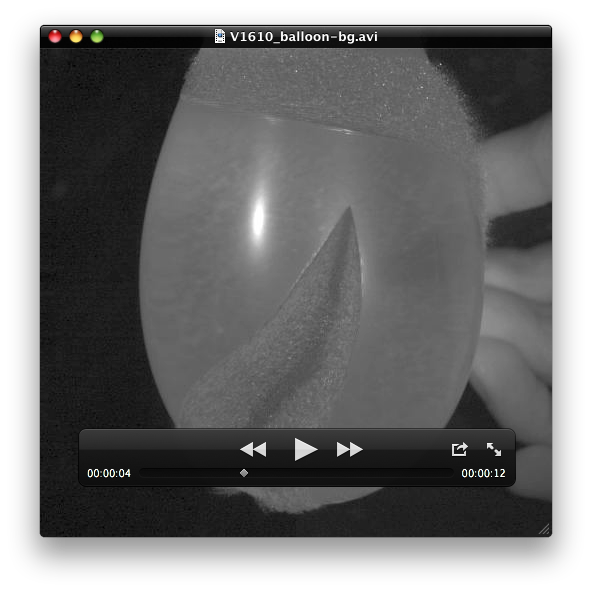
\includegraphics[width=2in]{figures/cine2avi_bg.png}
\end{tabular}

\vfill \pagebreak
\section{Using the CINE module in Python}
As an alternative to the command line tools, it is possible to use the \texttt{cine} module directly from your our \emph{Python} scripts.
This gives you an enormous flexibility in processing you images.

The following discussion assumes basic familiarity with \emph{Python} and the \emph{Scipy}/\emph{Numpy} pacakges.
For an introduction to using \emph{Python} for data analysis, \href{http://scipy.org/Getting_Started}{scipy.org} is a good resource.

At present, the \texttt{cine} module does not support color images for CINEs and TIFFs, but this will likely be included at some point in the future.

The most useful contents of the module are listed below, with a brief description:
\begin{itemize}
\item \texttt{Cine(FILENAME)}.  A class for reading CINE files. Loads frames on demand, so working with large CINEs (10's of GB) works fine.
\begin{itemize}
\item Frames can be accessed like items in a list, and return 2D arrays.  Iterating over the frames is also supported.
\item \texttt{len} returns the total number of frames.
\item Basic image properties appear as properties of the object, e.g. \texttt{frame\_rate}, \texttt{width}, \texttt{height}, \texttt{real\_bpp} (actual bit depth of the recorded image), and \texttt{shutter}.
\end{itemize}
\item \texttt{Tiff(FILENAME, ['r', 'w'])}.  A class for reading {\bf or} writing multi-page TIFFs.  %Create with the filename and read/write flag as options (only `r' {\bf or} `w' is supported).
\begin{itemize}
\item Supports only uncompressed, mono images with a bit-depth of 8--16 bits.
\item In read mode, frames accessed like list items.
\item In write mode, new pages are written to a TIFF with the \texttt{write\_page} function.
\end{itemize}
\item \texttt{Avi(FILENAME, [framerate=30], [quality=75])}. A class for {\bf writing} MJPEG AVIs.  Create with the filename.
\begin{itemize}
%\item Optional creation arguments are \texttt{framerate} [default: 30] and \texttt{quality} [0-100, default: 75].
\item New frames added with \texttt{add\_frame}, which accepts arrays or PIL images.
\end{itemize}
\item \texttt{Sparse} and \texttt{Sparse4D}. Classes for reading/writing sparse files.  Behave like \texttt{Cine} objects.
\item \texttt{open(FILENAME, )}. A generic command for opening CINE, TIFF, SPARSE of S4D images.  Returns the appropriate object.
\item \texttt{plot\_next\_to\_image(FRAME, [aspect=1])}. A functions that returns an array which is a combination of the original frame and the current \emph{Matplotlib} plot.  Height of plot will match image, and aspect ratio can be adjusted.
\item \texttt{asimage(FRAME)}.  A convenience function for turning an array into a PIL image.  Useful for saving single frames as images.
\end{itemize}

\vfill \pagebreak
\subsection{Basic Usage}
A \texttt{Cine} object is made by passing the filename to the \texttt{cine.Cine} class.
Once created, the class allows direct access to the image parameters and individual frames.
The below example was entered into an interactive prompt in \emph{Python}:

\begin{Verbatim}[commandchars=\\\{\}]
>>> import cine
>>> c = cine.Cine('V1610_balloon.cine')
>>> c.frame_rate \pyc{#Frames per second}
\textcolor{red}{49008}

>>> c.real_bpp \pyc{#Actual bits per plane}
\textcolor{red}{12}

>>> c.width, c.height \pyc{#Frame size}
\textcolor{red}{(512, 512)}

>>> len(c) \pyc{#Number of frames}
\textcolor{red}{379}

>>> \pyc{#Grab the 100th frame, convert to float with range (0-1)}
>>> frame = c[100].astype('f') / 2**c.real_bpp 
>>> frame.min(), frame.max()
\textcolor{red}{(0.011230469, 0.9921875)}

>>> frame_gamma = (frame - frame.min()) ** (1/2.2) \pyc{#Gamma correct}
>>> frame_8bit = (frame_gamma * 255).astype('u1') \pyc{#Convert to 8 bit}
>>> cine.asimage(frame_8bit).save('test.png') \pyc{#Convert to PIL image, save}
\end{Verbatim}

The following image was produced as \texttt{test.png}:

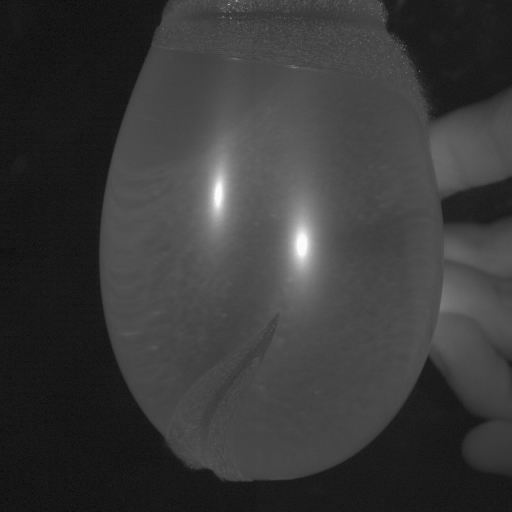
\includegraphics[width=2in]{figures/command_line_test.png}

\vfill \pagebreak
\subsection{Making an image array}
The following program imports a cine file, brightens a few frames and then exports them into a single image.


\begin{Verbatim}[frame=lines, label=example1.py, labelposition=topline, commandchars=\\\{\}]
\pyc{#!/usr/bin/env python}
from numpy import *
import cine

c = cine.open('V1610_balloon.cine') \pyc{#Equivalent to using cine.Cine}

minval, maxval = 60, 2000 \pyc{#Clip values}
gamma = 2.2

frames = []

for i in (50, 100, 150, 200):
    \pyc{#Resale minval-maxval to 0-1}
    f = (clip(c[i].astype('f'), minval, maxval) - minval) / (maxval - minval)
    
    \pyc{#Apply gamma correction and convert to 8bit (AKA 'u1')}
    frames.append((f**(1./gamma) * 255).astype('u1'))
    
cine.asimage(hstack(frames)).save('balloon_frames.png')
\end{Verbatim}

When run, this produces the following image:

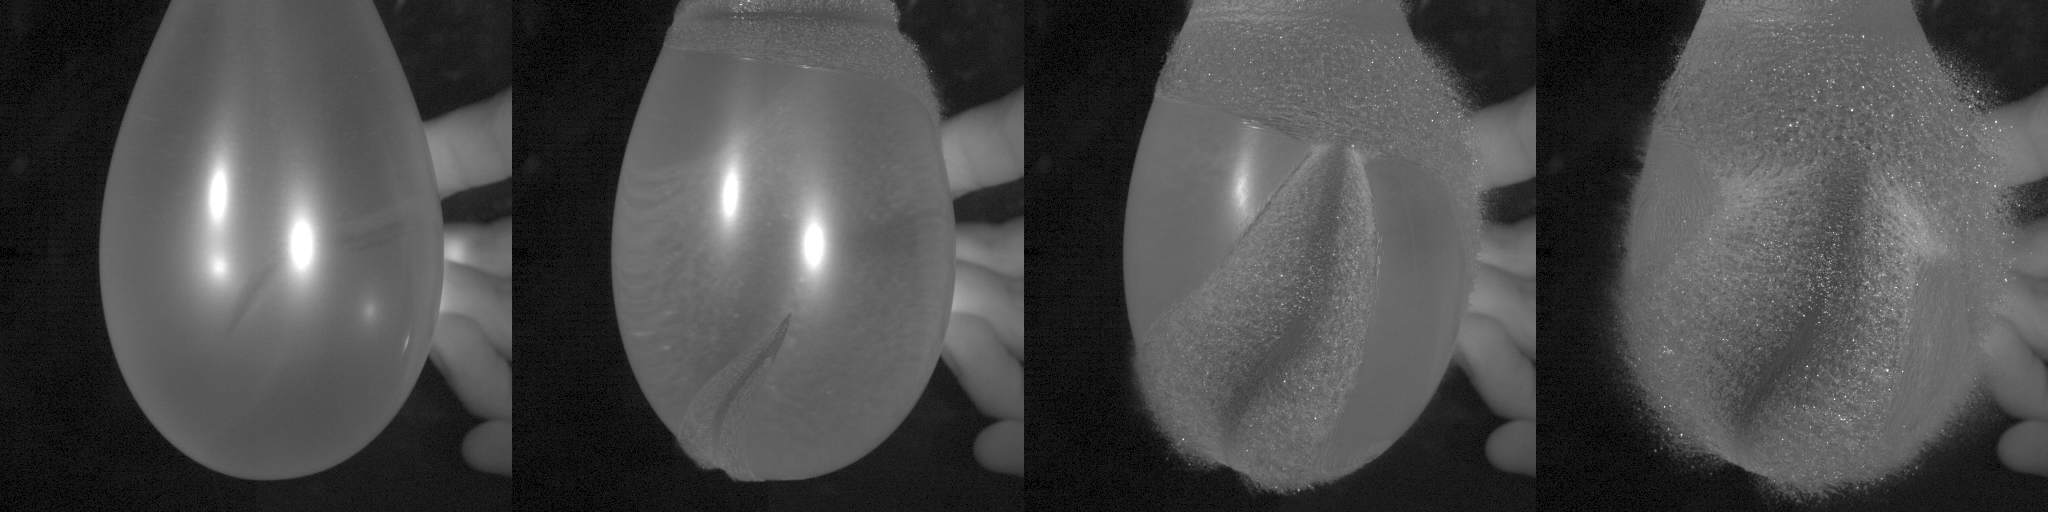
\includegraphics[width=6in]{figures/balloon_frames.png}

\vfill \pagebreak
\subsection{Producing an AVI with a Histogram}
Here we make use of \emph{Pylab} to make histogram plots, which we include alongside the original image and export to an AVI movie.

\begin{Verbatim}[frame=lines, label=example2.py, labelposition=topline, commandchars=\\\{\}]
\pyc{#!/usr/bin/env python}
from pylab import *
import cine

c = cine.open('V1610_balloon.cine') \pyc{#Equivalent to using cine.Cine}
minval, maxval = 60, 1000 \pyc{#Clip values}
bitmax = 2**c.real_bpp
gamma = 2.2
skip = 5 \pyc{#It's pretty slow to write every frame...}

\pyc{#Create new avi file}
output = cine.Avi('balloon_histo.avi', framerate=30./skip, quality=90)

for i in range(0, len(c), skip):
    \pyc{#Load frame, make histogram}
    f = c[i]
    count, bins = histogram(f, arange(0, bitmax, 4))
    
    \pyc{#Make the plot}
    semilogy(bins[:-1], count, '.')
    xticks([0, bitmax//4, 2*bitmax//4, 3*bitmax//4, bitmax-1])
    xlim([0, bitmax-1])
    ylim([1, 1E4])
    \pyc{#Shade the clipped region}
    fill_between([0, minval], [1, 1], [1E5, 1E5], facecolor='gray')
    fill_between([maxval, bitmax], [1, 1], [1E5, 1E5], facecolor='gray')
    title('Histogram (t = %5.3f ms)' % (1000.*i/c.frame_rate))
    xlabel('Pixel Value')
    ylabel('Counts')

    \pyc{#Clip frame, gamma correct}
    f = (clip(f.astype('f'), minval, maxval) - minval) / (maxval - minval)
    f = (f**(1./gamma) * 255).astype('u1')

    \pyc{#Create plot next to frame, and write to AVI}
    output.add_frame(cine.plot_next_to_image(f))
    close() \pyc{#close figure}

\end{Verbatim}

When run, an AVI is produced: 

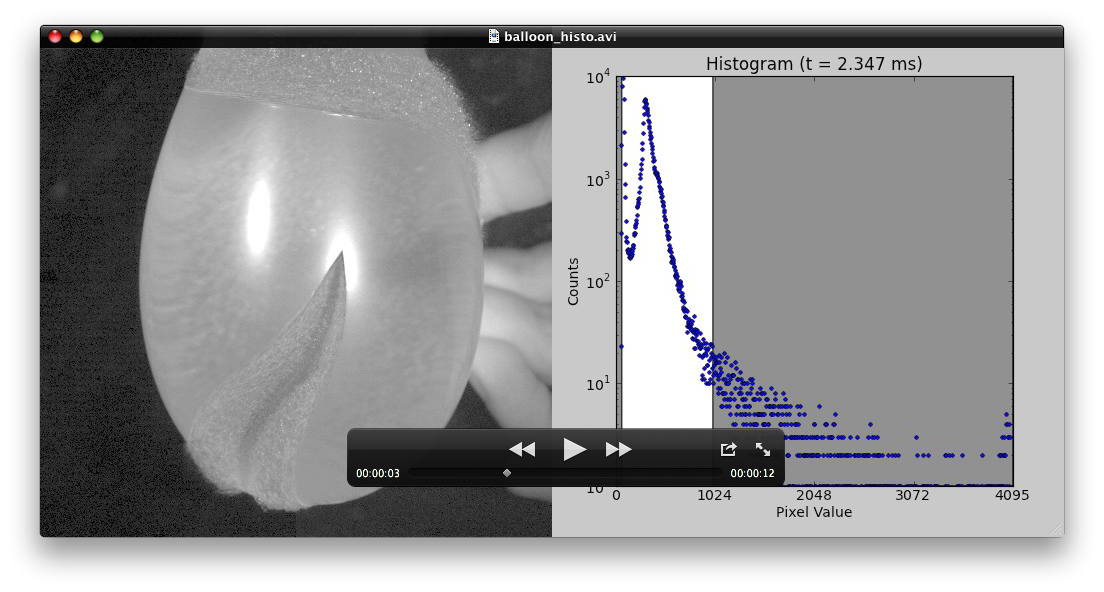
\includegraphics[width=6in]{figures/example2.png}


\end{document}  